\section{Numerical Examples}

In this section, we show you the results of implementing and experimenting with the methods described above. The implementation was done in julia=1.2.0. Code is made available in the github repository\footnote{\url{https://github.com/kw-lee/AdvStatComp_HDP}}.

\subsection{Cholesky Factorization}

The \textit{chol} function from \textbf{LinearAlgebra} package, the \textit{dpotrf} from \textbf{LAPACK} package, and hierarchical cholesky decomposition which suggested by \citet{hackbusch2015hierarchical} are implemented. Exponential covariance matrix, $\boldsymbol{\Sigma}_{ij}=exp(-\lVert \mathbf{s}_i-\mathbf{s}_j \rVert/\beta)$ is set with $\beta=0.3$. $n$ points, $\mathbf{s}_1,\cdots,\mathbf{s}_n$ is evenly distributed over unique square with Morton's order which defined recursively as described in figure \ref{fig:morton}.

\begin{figure}[ht]
\centering
	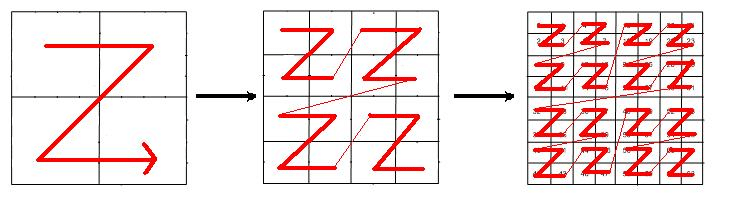
\includegraphics[width=.5\linewidth]{figs/Morton.jpg}
	\caption{Morton's order\citep{salem2016comparative}}
	\label{fig:morton}
\end{figure}

With various $n$, three Cholesky methods are applied and results are below table \ref{tab:table1}. In low rank approximation at algorithm \ref{alg:hchol}, rank is about $n^{1/4}$.

\begin{table}[!h]
	\centering
	% \resizebox{.6\textwidth}{!}{%
	{
		\begin{tabular}{@{}ccccc@{}}
			\toprule
			n & 256 & 1024 & 4096 & 16384 \\ \midrule
			chol & 0.001s & 0.0097s & 0.414s & 156.3s \\
			dpotrf & 0.0007s & 0.0132s & 0.431s & 154.1s \\
			hierarchical cholesky & 0.153s & 0.076s & 0.916s & 37.3s \\
			Error of hierarchical cholesky & 1.06e-7 & 9.97e-7 & 1.11e-3 & 1.87e-3 \\  \bottomrule
		\end{tabular}%
	}
	\caption{Excution times for Cholesky factorization}
	\label{tab:table1}
\end{table}
Hierarchical cholesky decomposition is more efficient than other classical cholesky method with large dimension. Hierarchical cholesky decomposition provides $\boldsymbol{\Sigma}\approx L_HL_H^T$. Its relative error is defined as $\frac{\lVert\boldsymbol{\Sigma}-L_HL_H^T\rVert_2}{\lVert\boldsymbol{\Sigma}\rVert_2}$, and table \ref{tab:table1} ensures accuracy of hierarchical cholesky decomposition proposed by \citet{hackbusch2015hierarchical}.


\subsection{Multivariate Normal Probabilities} 

To implement \texttt{*MVN} functions, we need to calculate $n$-dimensional normal probability \eqref{eqn:normalprob},
$$
\Phi_n(a, b; 0, \boldsymbol{\Sigma}) = \int_a^b \frac{1}{\sqrt{(2\pi)^n |\boldsymbol{\Sigma}|}} \exp\left( -\frac{1}{2} \mathbf{x}^T \boldsymbol{\Sigma}^{-1} \mathbf{x} \right) d\mathbf{x},
$$ 
numerically. We implement \texttt{mvn}, the function that calculate multivariate normal probabilities using Richtmyer QMC method introduced in subsection \ref{subsec:qmc}. Varying sample size $N$ and dimension $d$, two Monte Carlo methods are compared and results are below table \ref{tab:qmc_vs_mc}. We generate $N$ samples from $N(0, I_d)$ and set $\mathbf{a}_i = -\infty$ and $\mathbf{b}_i = 0$, i.e. true probabilities are $1/2^d$s, and repeat 20 times. Relative errors and computation times of each method are formulated.

\begin{table}[!h]
	\centering
	% \resizebox{.6\textwidth}{!}{%
	{
		\begin{tabular}{@{}cccccc@{}}
			\toprule
			$(n, d)$ 				  & 4 		& 8 	  & 12 		& 16 	  & 20	 \\ \midrule
			\multicolumn{6}{l}{Classical Monte Carlo} \\ \midrule
			\multirow{2}{*}{500}  & 12.2\%  & 56.8\%  & 161.9\% & 100.0\% & 100.0\% \\
								  & 0.294ms & 0.016ms & 0.018ms & 0.019ms & 0.019ms \\
			\multirow{2}{*}{1000} & 9.5\%   & 50.6\%  & 193.8\% & 100.0\% & 100.0\% \\
								  & 0.046ms & 0.041ms & 0.028ms & 0.028ms & 0.034ms \\
			\multirow{2}{*}{1500} & 8.9\%   & 38.7\%  & 150.2\% & 100.0\% & 100.0\% \\
								  & 0.055ms & 0.046ms & 0.042ms & 0.048ms & 0.045ms \\
			\multirow{2}{*}{2000} & 5.4\%   & 26.5\%  & 102.4\% & 100.0\% & 100.0\% \\
								  & 0.070ms & 0.065ms & 0.072ms & 0.058ms & 0.055ms \\
			\multirow{2}{*}{2500} & 5.1\%   & 32.0\%  & 100.1\% & 100.0\% & 100.0\% \\
								  & 0.073ms & 0.092ms & 0.081ms & 0.083ms & 0.076ms \\ \midrule
			\multicolumn{6}{l}{Richtmyer Quasi-Monte Carlo} \\ \midrule
			\multirow{2}{*}{500}  & 0.0\%   & 0.0\%   & 0.0\%   & 0.0\%   & 0.0\% \\
							      & 0.058ms & 0.003ms & 0.006ms & 0.006ms & 0.011ms \\
			\multirow{2}{*}{1000} & 0.0\%   & 0.0\%   & 0.0\%   & 0.0\%   & 0.0\% \\
						          & 0.003ms & 0.009ms & 0.013ms & 0.017ms & 0.020ms \\
			\multirow{2}{*}{1500} & 0.0\%   & 0.0\%   & 0.0\%   & 0.0\%   & 0.0\% \\
						          & 0.006ms & 0.011ms & 0.016ms & 0.019ms & 0.030ms \\
			\multirow{2}{*}{2000} & 0.0\%   & 0.0\%   & 0.0\%   & 0.0\%   & 0.0\% \\
						          & 0.011ms & 0.012ms & 0.013ms & 0.025ms & 0.036ms \\
			\multirow{2}{*}{2500} & 0.0\%   & 0.0\%   & 0.0\%   & 0.0\%   & 0.0\% \\
						          & 0.009ms & 0.022ms & 0.033ms & 0.038ms & 0.056ms \\ \bottomrule
		\end{tabular}%
	}
	\caption{Richtmyer Quasi-Monte Carlo and classical Monte Carlo}
	\label{tab:qmc_vs_mc}
\end{table}

Note QMC is superior to MC in every criterion. All the multivariate normal distribution probabilities required in the next algorithms are calculated using the \texttt{mvn} function.

\subsection{d-dimensional Conditioning Algorithm without/with Reordering}

Haar distribution is defined with a uniform distribution in the unitary $N\times N$ matrices group, $U(N)$.
\citet{stewart1980efficient} provides how to sample from Haar distribution with theorem \ref{thm:haar}

\begin{theorem}\label{thm:haar}\citet{stewart1980efficient}
	Let the independent vectors $x_1,\cdots,x_{n}$ be distributed $N(0,\sigma^2 \mathbf{I})$. For $j=1,2,\cdots,n-1$, let $\mathbf{\bar{H}}_{x_j}$ be the Householder transformation that reduces $x_j$ to $r_{jj}e_1$, where $r_{ij}$ is obtained in QR decomposition of $[x_1,\cdots,x_n]$ Let $\mathbf{H}_j=diag(\mathbf{I}_{j-1},\bar{\mathbf{H}}_j)$. Let $\mathbf{D}=diag(sign(r_{11}), \cdots, sign(r_{nn}))$. Then the product $\mathbf{Q}=\mathbf{DH_1\cdots H_{n-1}}$ follows Haar Distribution.
\end{theorem}

We simulates 250 MVN problems with various values of $m$ and $d$. $\boldsymbol{\Sigma}=\mathbf{Q}\mathbf{J}\mathbf{Q}^T$ is simulated with $\mathbf{Q}\sim{Haar distribution}$ and $J=diag(j_i)$ where $j_1,\cdots,j_m\sim U(0,1)$. Integration limits $a_i=-\infty$ and $b_i\sim(U,m)$ for $i=1\cdots,m$ are chosen. Estimated value is compared with approximated value obtained via quasi monte carlo method with a sample size of $10^4$, which ensures error below $10^{-4}$, and relative error and spent time is formulated below.

\begin{table}[!h]
	\centering
	% \resizebox{.6\textwidth}{!}{%
	{
		\begin{tabular}{@{}cccccc@{}}
			\toprule
			$(m, d)$ & 1 & 2 & 4 & 8 & 16 \\ \midrule
			\multicolumn{6}{l}{Without univariate reordering} \\ \midrule
			\multirow{2}{*}{16} & 3.7\% & 3.5\% & 3.6\% & 3.8\% & 2.9\% \\
			& 0.029ms & 0.201ms & 0.431ms & 0.676ms & 1.372ms \\
			\multirow{2}{*}{32} & 2.4\% & 2.9\% & 2.9\% & 3.3\% & 2.7\% \\
			& 0.001ms & 0.390ms & 0.833ms & 1.283ms & 2.545ms \\
			\multirow{2}{*}{64} & 1.9\% & 2.1\% & 2.1\% & 1.8\% & 1.9\% \\
			& 0.004ms & 0.762ms & 1.686ms & 2.545ms & 5.004ms \\
			\multirow{2}{*}{128} & 1.3\% & 1.5\% & 1.3\% & 1.2\% & 1.4\% \\
			& 0.024ms & 1.505ms & 3.333ms & 5.146ms & 10.548ms \\ \midrule
			\multicolumn{6}{l}{With univariate reordering} \\ \midrule
			\multirow{2}{*}{16} & 3.3\% & 3.1\% & 3.3\% & 3.6\% & 2.7\% \\
			& 0.007ms & 0.203ms & 0.439ms & 0.680ms & 1.363ms \\
			\multirow{2}{*}{32} & 2.3\% & 2.6\% & 2.6\% & 3.2\% & 2.6\% \\
			& 0.004ms & 0.393ms & 0.841ms & 1.289ms & 2.544ms \\
			\multirow{2}{*}{64} & 2.0\% & 2.1\% & 2.1\% & 1.9\% & 1.9\% \\
			& 0.014ms & 0.773ms & 1.695ms & 2.552ms & 5.022ms \\
			\multirow{2}{*}{128} & 1.2\% & 1.5\% & 1.4\% & 1.2\% & 1.4\% \\
			& 0.097ms & 1.593ms & 3.462ms & 5.268ms & 10.7861ms \\ \bottomrule
		\end{tabular}%
	}
	\caption{Errors and execution times of the d-dimensional conditioning method}
	\label{tab:table2}
\end{table}

Estimation error tended to decrease as $d$ increases with each $m$ since lager $d$ implers less discarded correlation information. Spent time grows to a linear fashion with m while it grows exponentially with $d$.

\subsection{Hierarchical-Block Approximations}
% HCMVN - 경원 (table 3)
% Block Reordering - 현석 (table 5, 6)

In this section, we implement three methods in the section \ref{sec:hmvn} and compare theirs performance
\begin{itemize}
    \item M1, \texttt{HMVN()}: Calculate multivariate normal probabilities using hierarchical-block approximation
    \item M2, \texttt{HCMVN()}: Calculate multivariate normal probabilities using hierarchical-block conditioning approximation
    \item M3, \texttt{HRCMVN()}: Calculate multivariate normal probabilities using hierarchical-block conditioning approximation with univarite reordering
\end{itemize}

We use 20 as the sample size instead of 250 as in Table \ref{tab:table2} because the covariance structure is fixed, leading to a much smaller standard deviation for the estimators. We simulates two spatial problems with various values of $m$ and $n$.

\begin{enumerate}
	\item Constant covariance matrix: $k(x_i, x_j) = \theta + (1-\theta)\delta_{ij}$ for some $|\theta| < 1$.
	\item 1D exponential covariance matrix: $k(x_i, x_j) = \exp(-d_{ij}/\beta)$ for some $\beta > 0$, where $d_{ij}$ is the distance between $x_i$ and $x_j$.
\end{enumerate}

We set the integration limits $a_i=-\infty$ and $b_i\sim(U,n)$ for $i=1\cdots,n$, $\theta=0.7$, $d_{ij} = 1$, and $\beta=10$ as in \citet{cao2019hierarchical}. Estimated value is compared with approximated value obtained via QMC with a sample size of $10^4$. In this simulation, we fix $d=4$ for \texttt{HCMVN} and \texttt{HRCMVN}. Table \ref{tab:table3} and Figure \ref{fig:table3_time} are errors and execution times under the constant covariance structure and 1D exponential covariance structure respectively. 

\begin{table}[!h]
	\centering
	{
		\begin{tabular}{@{}llllllllll@{}}
			\toprule
			$m$ 	& \multicolumn{3}{l}{16} & \multicolumn{3}{l}{32} & \multicolumn{3}{l}{64}  \\
			$n$ 	& 256 & 512 & 1024 & 256 & 512 & 1024 & 256 & 512 & 1024 \\ \bottomrule
			
			\multicolumn{10}{l}{Constant covariance structure} \\ \midrule

			M1 & 8.22\% & 7.11\% & 8.66\% & 8.94\% & 7.88\% & 6.68\% & 10.58\% & 8.05\% & 9.78\% \\
			M2 & 8.37\% & 7.08\% & 8.60\% & 8.91\% & 7.77\% & 6.61\% & 10.58\% & 8.26\% & 9.91\% \\
			M3 & 8.51\% & 7.10\% & 8.70\% & 9.51\% & 7.92\% & 7.00\% & 10.68\% & 7.94\% & 9.63\% \\

			\midrule
			
			\multicolumn{10}{l}{1D exponential covariance matrix} \\ \midrule

			M1 & 2.87\% & 0.00\% & 0.01\% & 0.07\% & 1.31\% & 0.00\% & 2.65\% & 0.27\% & 0.57\% \\
			M2 & 3.28\% & 0.01\% & 0.90\% & 0.07\% & 1.31\% & 0.01\% & 2.65\% & 0.28\% & 0.57\% \\
			M3 & 4.73\% & 0.09\% & 2.11\% & 2.17\% & 1.90\% & 0.16\% & 3.72\% & 1.25\% & 0.66\% \\
				
			\bottomrule
		\end{tabular}%
	}
	\caption{Relative errors under the constant covariance structure and 1D exponential covariance structure}
	\label{tab:table3}
\end{table}

\begin{figure}[!h]
	\centering
			\begin{subfigure}[b]{0.3\textwidth}
					\centering
					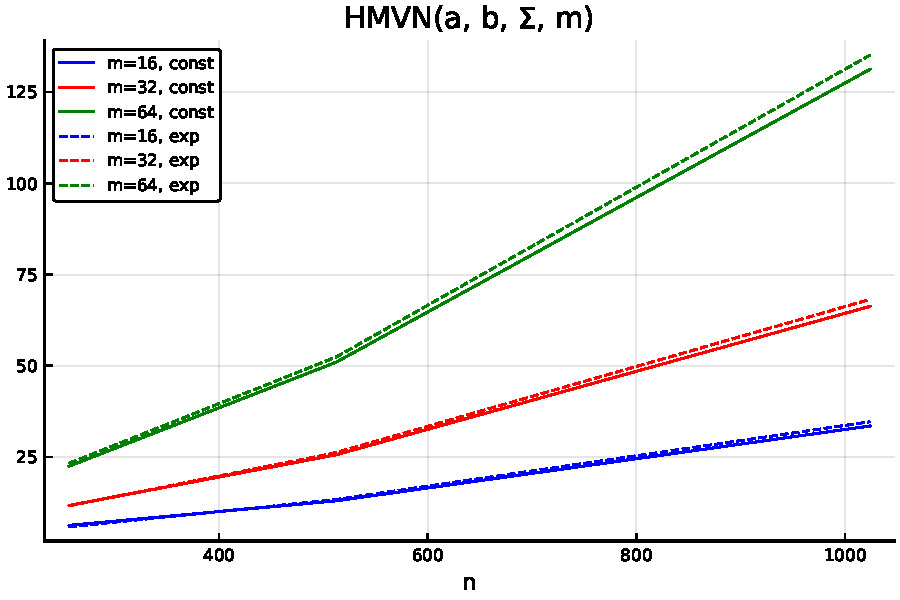
\includegraphics[width=\linewidth]{figs/table3_m1.pdf}
					\caption{M1}
			\end{subfigure}\hfill
			\begin{subfigure}[b]{0.3\textwidth}
					\centering
					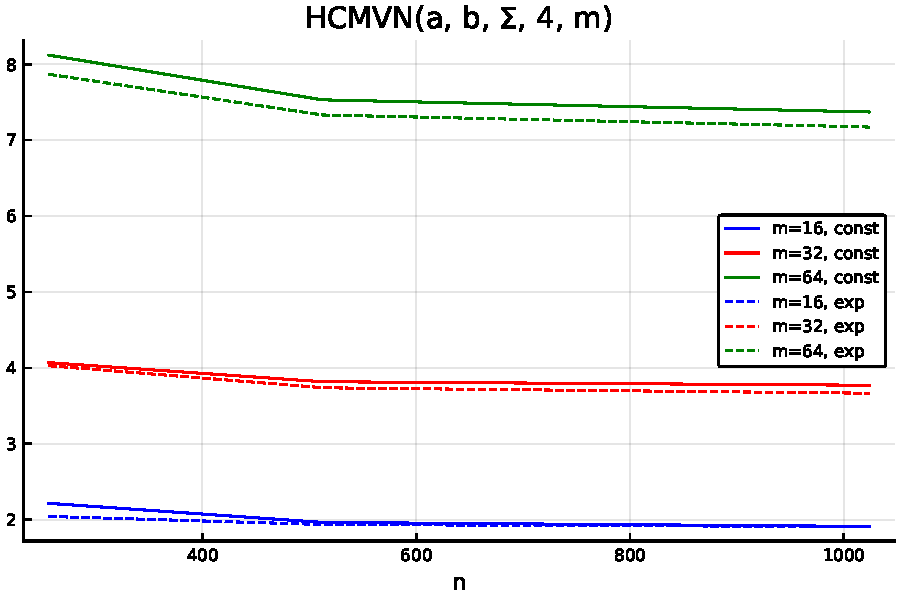
\includegraphics[width=\linewidth]{figs/table3_m2.pdf}
					\caption{M2}
			\end{subfigure}\hfill
			\begin{subfigure}[b]{0.3\textwidth}
					\centering
					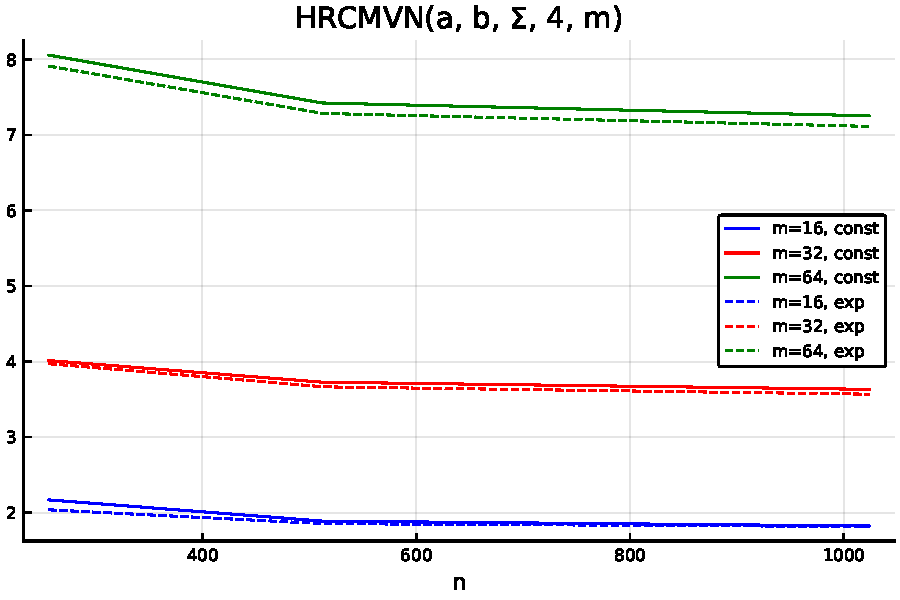
\includegraphics[width=\linewidth]{figs/table3_m3.pdf}
					\caption{M3}
			\end{subfigure}
			\caption{Execution time (seconds) under the constant covariance structure and 1D exponential covariance structure}\label{fig:table3_time}
\end{figure}	

Note the excution times of M2 and M3 are significantly smaller than of M1 even their performances are similar.

Next, we give simulation with a 2D exponential covariance matrix using morton's order for indexing the sample points on the plane. We fix $m = 8$ for the 2D covariance structure and examine the effectiveness of our algorithm varying $d =1,2,4$. To test the sensitivity with respect to the correlation strength, we perform the estimation under $\beta = 0.3, 0.1$, and 0.03, representing strong, medium, and weak correlation strengths. We set $n$ to 16, 64, 256 and other settings are same as above. Table \ref{tab:table5} presents the results.

\begin{table}[h]
	\centering
	{
		\begin{tabular}{@{}ccccccc@{}}
			\toprule
			$n$ & $compress$ & \texttt{mvn} & \texttt{HMVN} & $\texttt{HCMVN}_1$ & $\texttt{HCMVN}_2$ & $\texttt{HCMVN}_4$ \\ \midrule

			
			\multicolumn{7}{l}{$\beta=0.3$} \\ \midrule
			16 & 0.89 & 0.00ppm & 53.68ppm & 2139.98ppm & 1723.46ppm & 276.37ppm \\ 
			64 & 0.56 & 0.00ppm & 143.88ppm & 167.26ppm & 167.69ppm & 169.31ppm \\ 
			256 & 0.28 & 0.00ppm & 215.10ppm & 213.41ppm & 213.41ppm & 213.41ppm \\ 
			\midrule
			\multicolumn{7}{l}{$\beta=0.1$} \\ \midrule
			16 & 0.89 & 0.00ppm & 0.00ppm & 0.84ppm & 0.60ppm & 0.02ppm \\ 
			64 & 0.56 & 0.00ppm & 0.00ppm & 1.61ppm & 0.09ppm & 0.01ppm \\ 
			256 & 0.28 & 0.00ppm & 0.00ppm & 0.02ppm & 0.02ppm & 0.02ppm \\ 
			\midrule
			\multicolumn{7}{l}{$\beta=0.03$} \\ \midrule
			16 & 0.89 & 0.00ppm & 0.00ppm & 0.00ppm & 0.00ppm & 0.00ppm \\ 
			64 & 0.42 & 0.00ppm & 0.00ppm & 0.00ppm & 0.00ppm & 0.00ppm \\ 
			256 & 0.20 & 0.00ppm & 0.00ppm & 0.00ppm & 0.00ppm & 0.00ppm \\ 
			\bottomrule
		\end{tabular}%
	}
	\caption{Relative errors and efficiency of the two-level hierarchical-block conditioning methods}
	\label{tab:table5}
\end{table}

\begin{figure}
	\centering
	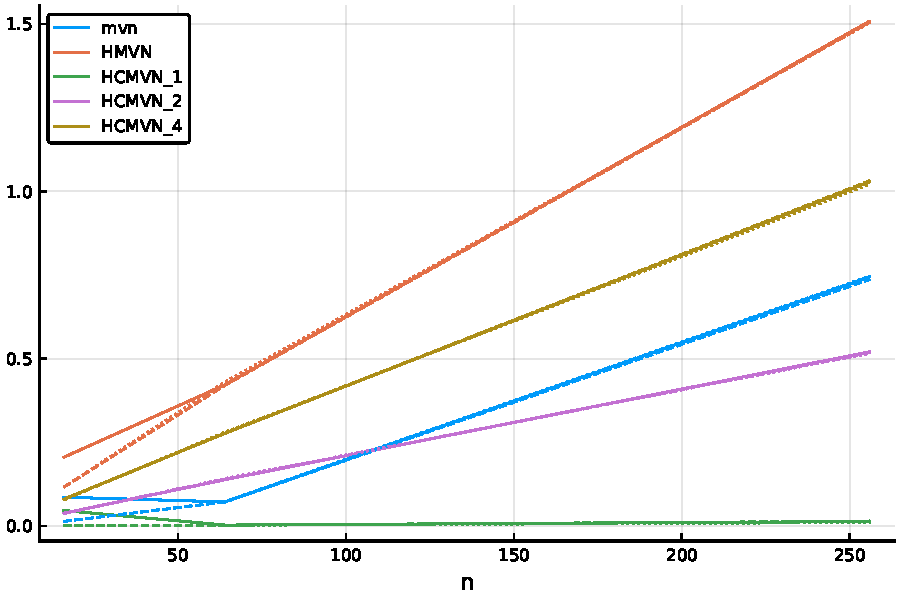
\includegraphics[width=0.7\linewidth]{figs/table5_time.pdf}
	\caption{Execution time (seconds) under the constant covariance structure and 2D exponential covariance structure; solid line: $\beta=0.3$, dashed line: $\beta=0.1$, dotted line: $\beta=0.03$}\label{fig:table5_time}
\end{figure}

In Table \ref{tab:table5}, $\texttt{HCMVN}_d$ denotes \texttt{HCMVN} function with conditioning parameter $d$ and  
$$compress = \frac{\text{Total memory size of the } \mathcal{H} \text{ matrix}}{\text{Memory size of the covariance matrix } \boldsymbol{\Sigma}}.$$ 

In this experiment, \citet{cao2019hierarchical} mentioned 
\begin{quote}
	It is worth mentioning that the correlation strength is essentially increased when $n$ increases while $\beta$ remains unchanged because the samples are from the unit hypercube. Also the increase of $d$ will reduce the estimation error but is still unable to reach a satisfactory level. The method, when used without a reordering strategy, does not produce sufficiently accurate results. This motivated the development of the reordering strategy described in the next section
\end{quote}
with extremely large size simulation. But, in our experiment, above phenomenon could not be observed due to restriction of the computing resource.

% \subsection{Block Reordering}
% Block Reordering - 현석 (table 5, 6)
